\chapter{System Evolution and Design Decisions}
\label{chap:evolution}

\begin{chapterplan}{14--17 pages}{Explain how the system changed in response to observed technical weaknesses, and distinguish implemented ideas from runtime behaviour and measured effects.}
The chapter reconstructs the main engineering decisions from project records and the archived repository. It reports what can be demonstrated and identifies where a proposed correction was not yet connected or evaluated.
\end{chapterplan}

\section{Purpose, Scope, and Evidence Standard}
\label{sec:evolution-purpose}

The architecture was not designed in one pass. It changed whenever the prototype exposed a practical problem. Dense vector search and procedural Blender output came first; lexical retrieval, deduplication, image search, storage abstraction, a geometry catalogue, and an MCP boundary followed later. Some of those changes became part of the active route, while others stopped at a branch or partial integration. I reconstruct that history because the unsuccessful and unfinished approaches explain the final design as much as the retained components do.

Rather than repeat a fixed checklist for every decision, I follow the sequence in which the problems became visible. The account asks what evidence was available at the time, why one correction was chosen, and what remained unresolved afterwards. That form of reflection is consistent with design-science research, where building and evaluating an artefact can produce knowledge about both the proposed solution and its context \parencite{hevner2004,peffers2007,wieringa2014}.

Four evidence levels are used. Project notes and formative evaluations support the historical account. Repository files show implementation. Call-graph inspection is required before a mechanism can be described as part of an endpoint, and a controlled run is required before any performance effect is claimed. The hybrid retriever is a useful example: the source code exists, but the archived production path did not instantiate it. Historical material comes mainly from \codepath{project_resources/THESIS_SYSTEM_DESIGN_AND_MCP.md}, \codepath{project_resources/EVALUATION_DATA_SUMMARY.md}, and \codepath{project_resources/PROFESSOR_REQUIREMENTS_TRACEABILITY.md}; implementation statements are checked against the repository.

\begin{figure}[htbp]
  \centering
  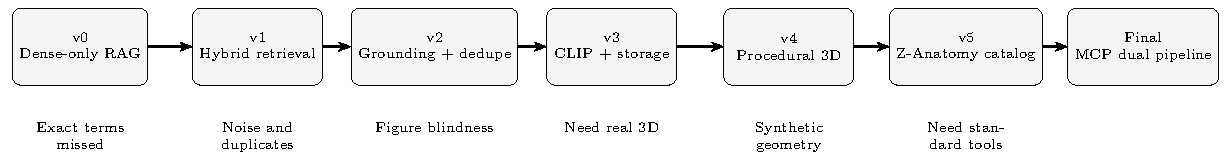
\includegraphics[width=\textwidth,height=0.45\textheight,keepaspectratio]{figures/rendered/evolution_timeline.pdf}
  \caption{High-level evolution from the dense-only prototype to the separated RAG and MCP architecture. The sequence represents design development, not measured performance.}
  \label{fig:evolution-timeline}
\end{figure}

\section{Evolution of the Document-Grounded RAG Pipeline}
\label{sec:evolution-rag}

\subsection{Initial Monolithic Dense-Only RAG}
\label{sec:evolution-dense-baseline}

The first working document route was deliberately conventional. PDF text was chunked, encoded as dense vectors, stored in Chroma, retrieved by similarity, and inserted into the language-model prompt \parencite{reimers2019,karpukhin2020}. This gave the project an end-to-end baseline without requiring domain-specific training data or several ranking stages at once. Its lineage is still visible in \codepath{src/ingestion/run.py}, \codepath{src/retrieval/vector_store.py}, and \codepath{src/multimodal/multimodal_rag_chain.py}.

Its value became clearest when it failed. Exact anatomy terms were handled inconsistently, near-identical references accumulated in the interface, and plausible answers were built from passages that mentioned the topic without answering the question. Figure-centred questions exposed the limits of the text-only index as well. These problems initially looked like model failures, but the records pointed to a wider chain involving extraction, retrieval, candidate selection, prompt construction, and source presentation.

Instead of replacing or fine-tuning the generator immediately, the project separated the pipeline into smaller, inspectable concerns. That choice led to the later work on lexical retrieval, deduplication, grounding, image support, and asset delivery. Because no dated snapshot fully reproduces the earliest baseline, I use it as a documented development stage rather than a formal comparison condition.

\subsection{Dense Retrieval to BM25, Dense Search, and RRF}
\label{sec:evolution-hybrid-retrieval}

Dense retrieval remained useful for questions that paraphrased the source. At the same time, anatomy contained distinctions that depended on the exact token: left or right, a short abbreviation, a Latin label, or a named structure. This led to \codepath{src/retrieval/hybrid_retriever.py}, which combines dense candidates with BM25, phrase matching, and weighted Reciprocal Rank Fusion \parencite{karpukhin2020,robertson2009,cormack2009}.

RRF offered a simple way to combine rankings without averaging incompatible dense and lexical scores. It also kept the prototype understandable and avoided the need for a labelled training set. Domain-specific embeddings, cross-encoders, and query expansion remained possible alternatives, but they would have added data requirements or latency before the basic orchestration was stable.

Repository inspection refined the interpretation of this work. The hybrid class was connected to the production \codepath{MultimodalRAG} path in commit \texttt{5089fcc} (12~July~2026). An earlier dense-only snapshot (\texttt{cb041d5}, 27~June~2026) remains historical context. Hybrid retrieval is therefore reported as the hybrid-preferred production route used by the primary July evaluation, not as a proven improvement over dense-only retrieval: a matched comparison is still required for this corpus and question set. The episode established a reporting rule that I use throughout the thesis: source code, active runtime behaviour, and measured effect are different claims.

\subsection{Duplicate Passages, the Early Three-Source Rule, and Later Type-Dependent Caps}
\label{sec:evolution-deduplication}

A separate problem appeared in the evidence shown to users. Overlapping chunks, repeated ingestion, filename variants, and duplicate pages could make the same underlying text look like several independent sources. Increasing the candidate count only lengthened the prompt and made the source cards less informative.

In an earlier design stage, the dense-only RAG chain retrieved up to 24 text candidates, removed repeated text fingerprints and duplicate source--page pairs, and retained at most three passages. That hard three-passage rule was a usability choice introduced to reduce clutter and repeated citations, not an experimentally derived optimum. \codepath{src/multimodal/multimodal_rag_chain.py} still uses a SHA-256 fingerprint of roughly the first 220 normalised characters together with normalised PDF stems and page identity; image candidates are also capped and deduplicated.

After hybrid retrieval was connected to the production route, the evaluated July implementation no longer applied that fixed cap as the active default. Final context size was selected by question type through \codepath{max_passages_for_type}, yielding approximately four to eight unique passages. Shorter evidence sets remain easier to read and cite, but multi-part questions may need more support. The source--page rule can also collapse distinct material from the same page, and duplicate vectors may remain in the store. The underlying lesson is that a top-$k$ list is merely a ranking; it is not automatically a set of independent evidence. The hard three-passage rule is therefore preserved as design history; it is not described as active in the primary July evaluation.

\subsection{Weak Evidence, Evidence Grading, and Abstention}
\label{sec:evolution-grounding-controls}

Formative evaluation exposed a more serious issue. A passage could mention the correct structure without answering the question, yet the generator would still produce a fluent explanation. The project had treated retrieval relevance too readily as evidence sufficiency. This reflects a known limitation of RAG: external context can reduce unsupported generation without preventing it \parencite{lewis2020,ji2023}.

The response was a set of controls under \codepath{src/rag/}: evidence grading, numbered-passage prompts, citation filtering, answer verification, query policy, and quotation handling. The stricter \codepath{/rag/experiment/ask} route passes numbered evidence to a constrained prompt. Its intended sequence is to grade the retrieved material, admit only adequate passages, and abstain or request consent when the documents cannot support an answer.

The production route never completed that integration. In the archived snapshot, \codepath{AskRequest} accepts only the question; language and world-knowledge fields sent by the frontend are ignored, and fallback to general knowledge remains possible. That interface mismatch has behavioural consequences because an unused policy field cannot constrain the response. The records contain unsupported answers but no controlled before-and-after abstention study. I therefore describe evidence grading and strict prompting as implemented mechanisms with incomplete production wiring. They also create their own evaluation needs, including grader error, over-refusal, and span-level checks for exact quotation.

\subsection{Figure Blindness and CLIP}
\label{sec:evolution-clip}

Questions centred on figures exposed a limitation that text retrieval could not solve. Anatomy documents contain diagrams, histology, radiology, and labelled views in which the image carries information that nearby prose only partly captures. The ingestion route was extended to extract images and retain their metadata. A separate CLIP index then supports text-to-image retrieval, followed by reranking, deduplication, and optional URL return \parencite{radford2021}.

Text and image representations were kept separate because MiniLM and CLIP operate in different spaces and their scores are not directly comparable. Late fusion made the behaviour easier to inspect: the document route could return passages and an answer, while the image route supplied candidates without pretending that one number ranked both modalities.

The application could now return figures, but this was only an integration result. Project notes record irrelevant matches, and the general-domain CLIP model may miss fine anatomical distinctions or small labels. PDF extraction can split composite figures, while remote-only records may depend heavily on captions or nearby text. What began as ``add a vision encoder'' became a broader delivery problem involving extraction, metadata, ranking, duplicates, provenance, and browser access.

\subsection{Local Paths and Storage Abstraction}
\label{sec:evolution-storage}

The first image implementation failed at the point of delivery. A correct local filename was not necessarily a URL that a browser, another container, or a remote client could fetch. Paths that worked on the development machine broke after restart or deployment because retrieval identity and delivery location had been stored together.

\codepath{app/services/object_storage.py} separated those concerns by adding stable object keys, provider-specific upload logic, presigned URLs for MinIO or Supabase, and diagnostics. A local static fallback remained for development. The same retrieval record could then be resolved according to the deployment environment rather than a hard-coded path.

Portability improved, but the operational risks remained. Signed URLs expire, credentials and buckets can be misconfigured, and a local fallback is unsuitable for several replicas. Copyright-sensitive material also restricts which storage provider is appropriate. In practice, image retrieval is not complete until the chosen asset can be delivered under the intended deployment conditions.

\section{Evolution of the 3D Anatomy Pipeline}
\label{sec:evolution-3d}

\subsection{Procedural Blender and Synthetic Geometry}
\label{sec:evolution-procedural-blender}

The first Blender experiment generated a brain-like form from primitive meshes in \codepath{src/mcp/blender_generator.py}. Its purpose was infrastructural: confirm that the backend could launch Blender in headless mode and write GLB and PNG files. Anatomical detail was not the priority at that stage.

That experiment also exposed the weakness of file creation as a success criterion. A mesh could be technically valid and visually plausible while lacking accepted anatomy, traceable labels, or any link to the teaching material. Further procedural modelling would have shifted the project towards asset production, while commercial assets would have introduced licensing and reproducibility concerns.

The procedural route was retained only as evidence that the infrastructure worked. The educational path moved to existing Z-Anatomy geometry. Because the legacy endpoint still exists, architecture descriptions must name it explicitly; otherwise the synthetic experiment can be mistaken for the catalogue-based MCP workflow.

\subsection{Remote Preview Worker Limitations}
\label{sec:evolution-preview-worker}

A remote preview worker served as an intermediate solution. It mapped a small vocabulary, such as brain or heart, to predefined assets and returned a rendered PNG beside the RAG answer. This added a visual element at modest cost and avoided arbitrary access to the Blender scene.

The limits appeared quickly. A fixed map could not handle a request such as \texttt{left femur}, and a PNG was neither interactive nor labelled. Adding more keywords would have increased maintenance without changing the closed nature of the interface. The worker remained an optional RAG adjunct, while open-ended structure requests moved to a separate mode.

The archived \codepath{app/services/rag_service.py} still calls this worker after RAG generation, and \codepath{app/services/blender_service.py} contains the fixed asset map. A final evaluation must disable it or report it separately. A successful preview says nothing about MCP catalogue resolution or export of the requested geometry.

\subsection{Adoption of Z-Anatomy}
\label{sec:evolution-zanatomy}

Adopting Z-Anatomy changed the task. Blender no longer had to invent a form; the application could select named objects from an existing anatomy scene and export them with annotations \parencite{zanatomy}. This gave the artefact a traceable source and made repeated exports possible from the same \codepath{Startup.blend} file.

An existing scene did not make language resolution simple. Blender object names and collection hierarchies are designed for scene management, not student questions. Aliases, laterality, broad terms, and structures represented by several objects all created ambiguity. Exporting the entire scene would have avoided selection but produced unwieldy results, while unconstrained LLM selection would have weakened reproducibility. The project paired the scene with an offline catalogue and constrained resolver instead.

Configuration, scene scanning, export scripts, static mounts, and the Three.js viewer are present under \codepath{anatomy_mcp/}, which establishes the implementation path. The exact Z-Anatomy release, source hash, licence record, and local modifications were not frozen with the evaluation package. Provenance narrows uncertainty, but it cannot certify the anatomical completeness of every selected object.

\subsection{Raw Scene Labels versus the Exportable Catalogue}
\label{sec:evolution-exportable-catalog}

The first scene index, \codepath{z_anatomy_index.json}, recorded names from the Blender file. It improved search, but a name might still refer to an empty collection, an unsuitable hierarchy node, or an excessively broad object set. Project records contain empty and oversized matches; the earlier left-femur example made laterality and scope especially visible.

The replacement, \codepath{exportable_catalog.json}, was built offline with object type, side, hierarchy, bounding-box, and geometry metadata. \codepath{anatomy_mcp/blender_scripts/build_exportable_catalog.py} records exportability information, and \codepath{anatomy_mcp/catalog_search.py} performs token- and side-aware matching. A basic capability check can therefore occur before the costly Blender call.

The catalogue is more useful than a raw label list, although its meaning is still technical. \texttt{Femur.l} is a scene identifier rather than standard anatomical nomenclature, and a non-empty bounding box cannot show that the geometry is complete or educationally appropriate. Manual curation and learned entity linking remain future options. The important boundary is that a side-effecting tool searches a set of validated capabilities rather than every name found in the scene.

\subsection{Direct Python Calls versus MCP Stdio}
\label{sec:evolution-mcp}

Direct Python calls connected the backend to export functions quickly, but interpretation, tool choice, and Blender execution remained inside one application process. The interface was specific to the codebase and provided little protocol-level evidence about which capability had been discovered or invoked.

The later design introduced a FastMCP server, stdio transport, an MCP \codepath{ClientSession}, tool discovery, and \codepath{call_tool}. MCP supplies a structured host--client--server contract for bounded tools and schemas \parencite{mcp20250618}. In the archived code, \codepath{app/services/anatomy_mcp_client.py} launches the server, lists tools, and invokes them. \codepath{anatomy_mcp_chat.py} then uses a deterministic fast path for simple labels and an LM Studio tool loop for more complex phrasing.

HTTP services, queues, or custom JSON-RPC could also isolate Blender, but they would not satisfy the MCP research objective. Local stdio provided process separation without another network service and let simple requests avoid unnecessary model rounds. The code demonstrates real MCP initialisation and execution, although runtime success still depends on compatible SDK versions, valid paths, Blender, and a tool-capable model for the LLM loop.

\subsection{Fake 3D Success versus Model-URL Verification}
\label{sec:evolution-artifact-verification}

One failure became particularly clear: assistant prose had been treated as proof that an export occurred. Earlier flows could report success even when no usable GLB or viewer existed. The correction was to make structured output authoritative. \codepath{structured_to_anatomy_export} rejects a success result without \codepath{model_url}, and the viewer is intended to render only a verified export object.

A model URL is only the minimum practical check. Stronger validation would cover file existence and size, GLB structure, selected-object logs, annotation parsing, HTTP retrieval, and visual correctness. The archived frontend contains a compatibility path in \codepath{AnatomyMcpPanel.js} that reconstructs export data from URLs in assistant text. Because this partly restores the weakness that structured output was meant to remove, it should be disabled during evaluation.

This changes the evidential standard. A conversational message may explain the result, but only an observable tool result and accessible artefact can establish technical success. Anatomical correctness then requires a separate check of what was resolved and exported.

\subsection{Blender Locking and Cache}
\label{sec:evolution-lock-cache}

Blender export is neither lightweight nor stateless. A request may open a large scene, select objects, write several files, and compete for paths or process resources. Project notes recorded intermittent failures and repeated waiting when this behaviour was left uncontrolled.

\codepath{anatomy_mcp/server.py} addresses this with a module-level \codepath{RLock} and versioned cache keys for models, annotations, previews, and packages. \codepath{anatomy_mcp/config.py} records schema version \codepath{v4}, and tool responses expose \codepath{cache_hit}. For a single-machine prototype, a process-local lock and cache were proportionate and easier to inspect than a queue or worker fleet.

The controls introduce their own limitations. The lock serialises work and cannot coordinate separate server processes. Cache value depends on invalidation after changes to the scene, catalogue, exporter, or options. Because no concurrency test or cold-versus-cached benchmark was completed, I report the mechanism and its rationale rather than a quantified gain.

\section{From Mixed Responsibilities to Independent Pipelines}
\label{sec:evolution-dual-pipeline}

As the two feature sets grew, the broad label ``anatomy chatbot'' became misleading. Failures could originate in PDF extraction, retrieval, generation, catalogue resolution, Blender, storage, or the viewer, while one chat surface hid the distinction. The redesign introduced separate panels and FastAPI endpoints: \codepath{/rag/ask} for document questions and \codepath{/anatomy/ask} for 3D requests.

This was a compromise. Two separate applications would duplicate infrastructure and fragment the user experience; automatic intent routing through one chat box would hide the applicable source and success condition. Separate panels retained a shared shell while making the selected mode visible to both user and evaluator.

The archived snapshot is not completely separated. The RAG service still calls the fixed preview worker from the earlier adjunct design, so it must be disabled, labelled, or excluded from MCP scoring. This showed that folder structure alone does not create modularity. Each mode needs its own input contract, source of truth, failure semantics, evidence, and metrics.

\section{Cross-Cutting Lessons}
\label{sec:evolution-cross-cutting-lessons}

Across both pipelines, indirect proxies were gradually replaced by inspectable evidence. A lexical branch supplemented dense similarity; repeated retrieval records were reduced before display; weak passages prompted stricter evidence handling; synthetic geometry gave way to a defined anatomy source; the raw scene index became an exportability catalogue; and conversational success was replaced by a structured artefact contract. These changes made the system easier to analyse even when their performance effect had not been measured.

The recurring difficulty was drift between design, code, and orchestration. Hybrid retrieval became the preferred production path, yet world-knowledge consent and some stricter grounding controls remain incomplete on \codepath{/rag/ask}. The frontend sends fields that the backend ignores, and the URL-salvage path weakens the 3D contract. These are not peripheral inconsistencies; they determine which system the evaluation actually describes.

The 3D branch adds another limitation. MCP improves traceability of the process, but it cannot decide whether the chosen anatomy is correct. That judgement still depends on query interpretation, laterality, catalogue coverage, object selection, export validity, and the viewer. A dataset label may identify the selected object without showing that it is complete or educationally suitable.

\section{Consolidated Design-Decision Matrix}
\label{sec:evolution-matrix}

\begin{landscape}
\tiny
\setlength{\tabcolsep}{2.5pt}
\renewcommand{\arraystretch}{0.72}
\begin{table}[p]
\centering
\caption{Consolidated design-decision matrix. ``Implemented'' denotes repository evidence, not verified production execution or measured improvement.}
\label{tab:decision-matrix}
\begin{tabularx}{\linewidth}{L{0.12\linewidth}L{0.17\linewidth}L{0.21\linewidth}L{0.21\linewidth}Y}
\toprule
Theme & Initial design & Observation & Selected correction & Evidence status and residual limitation \\
\midrule
Retrieval & Dense search only & Exact terminology was weakly handled & BM25, dense search, phrase matching, and RRF on the production path & Hybrid preferred after \texttt{5089fcc}; matched dense ablation missing \\
Evidence selection & Unfiltered top-$k$ passages & Repeated chunks and citation sprawl & Deduplication; early hard three-source rule; later type-dependent caps & Early three-source rule historical; July caps approx.\ 4--8 \\
Grounding & Permissive synthesis & Unsupported answers from weak context & Grading, strict prompts, citation checks, and abstention & Modules exist; production integration incomplete \\
Multimodality & Text-only index and local paths & Figure blindness and inaccessible assets & CLIP retrieval and storage abstraction & Implemented; relevance and URL reliability unmeasured \\
Early 3D & Procedural mesh and fixed previews & Synthetic provenance and limited vocabulary & Z-Anatomy source geometry & Source path exists; legacy routes remain \\
Resolution & Raw scene labels & Names did not guarantee bounded geometry & \codepath{exportable_catalog.json} & Implemented; exportability is not anatomy correctness \\
Tool execution & Direct calls and prose success & Weak auditability and unverifiable claims & MCP stdio and artefact verification & MCP tools exist; URL salvage should be disabled \\
Operations & Parallel uncached export & Reported instability and repeated waiting time & Process-local lock and versioned cache & Implemented; multi-process safety and effects unmeasured \\
Architecture & Mixed responsibilities & Unclear failure ownership and metrics & Independent RAG and MCP interfaces & Separation exists; preview worker remains in RAG \\
\bottomrule
\end{tabularx}
\end{table}
\renewcommand{\arraystretch}{1.0}
\normalsize
\end{landscape}

\section{Evidence Checklist Before Final Claims}
\label{sec:evolution-evidence-checklist}

Stronger performance claims require the following evidence:

\begin{enumerate}[leftmargin=*,itemsep=0.15em,topsep=0.3em]
  \item archive the repository commit, corpus hashes, prompts, model revisions, and environment used for evaluation;
  \item retain the hybrid-preferred route as the production default and run a matched dense-versus-hybrid comparison;
  \item save candidate and final source identifiers so that deduplication can be evaluated rather than inferred;
  \item define expected behaviour for unsupported, off-topic, typo, and quotation cases and retain the raw traces;
  \item create an expert-labelled figure subset covering relevance, duplicates, provenance, and broken URLs;
  \item record the Z-Anatomy release, licence, source hash, local modifications, and catalogue-generation log;
  \item test exact labels, aliases, laterality, ambiguity, and invalid catalogue requests while preserving selected-object evidence;
  \item retain MCP tool traces, success and failure JSON, GLB checks, annotation parsing, and viewer evidence;
  \item measure cold and cached latency and exercise concurrent requests; and
  \item keep RAG and MCP result sheets separate, with the preview worker and URL-salvage path isolated during evaluation.
\end{enumerate}

The implementation account in \cref{chap:implementation} must stay aligned with the evaluated runtime. Hybrid retrieval, consent handling, strict evidence grading, and complete separation should be described as production behaviour only after their call paths have been verified.

\section{Chapter Summary}
\label{sec:evolution-summary}

The development moved from a convenient demonstration towards a system whose outputs could be inspected. Dense-only retrieval revealed lexical and evidence-selection weaknesses. Figure questions forced the project to handle a second modality and the delivery of extracted assets. Procedural Blender output proved execution but lacked anatomy provenance, which led to Z-Anatomy, an exportability catalogue, and an MCP boundary. Artefact verification, locking, caching, and separate interfaces addressed failures that prompt design alone could not solve.

Several corrections remain incomplete at runtime or in evaluation. The archived production endpoint does not fully connect the hybrid and grounding components, and frontend compatibility behaviour weakens the strict export contract. These gaps are part of the result because they identify what must change before the prototype can be evaluated as the system shown in the architecture.

The final separation grew from those observations. Document answers require retrieval, support, citation, and boundary checks. Three-dimensional requests require catalogue resolution, tool traces, valid files, viewer checks, and explicit failure states. Treating them as different evidence problems makes the architecture easier to defend and the unfinished work easier to specify.
